\section{Hadoop Open Platform-as-a-Service (Hops)}
\label{hops}

A full installation of our platform builds on an adapted distribution of the Hadoop File System (HDFS), called HopsFS, which builds on a new metadata management architecture based on a shared-nothing, in-memory distributed database (see Figure \ref{fig:hops}). Provided enough main memory in the nodes, metadata can  grow to TBs in size with our approach (compared to  ~100GB in Apache HDFS \cite{shvachko2010Hdfs}), which allows HopsFS to store 100s of millions of files. The HopsFS architecture includes multiple stateless NameNodes that manage the namespace metadata stored in the database (see Figure \ref{subfig:hopsfs}). HopsFS' clients and DataNodes are aware of all NameNodes in the system. HopsFS is  highly available: whenever a NameNode fails the failed operations are automatically retried by clients and the DataNodes by forwarding the failed requests to a different live NameNode. We use MySQL Cluster~\cite{ronstrom2005recovery} as the database, as it has high throughput and is also highly available, although any distributed in-memory database that supports transactions and row level locking could be used. On database node failures, failed transactions are re-scheduled by NameNodes on surviving database nodes.

\begin{figure}[!ht]
    \subfloat[HopsFS\label{subfig:hopsfs}]{%
      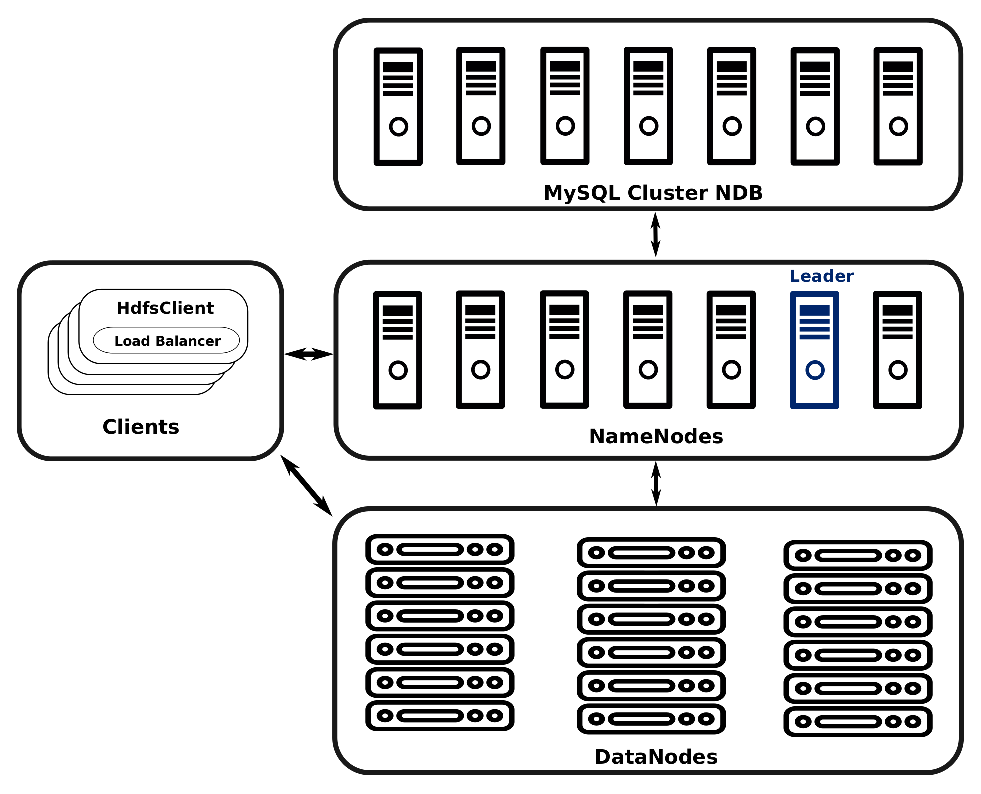
\includegraphics[width=0.46\textwidth]{./imgs/hops-fs-arch.eps}
    }
    \hfill
    \subfloat[HopsYARN\label{subfig:hopsyarn}]{%
      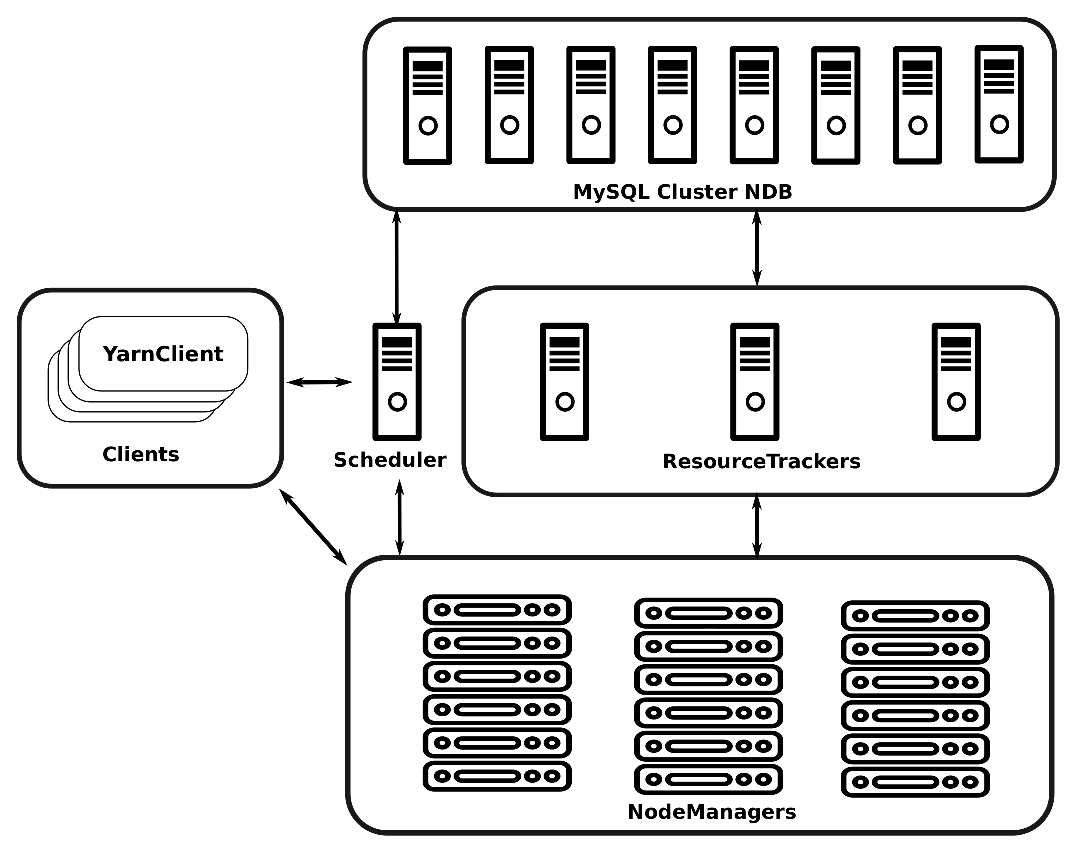
\includegraphics[width=0.47\textwidth]{./imgs/hops-yarn-arch.eps}
    }
    \caption{HopsFS and HopsYARN architectures.}
    \label{fig:hops}
\end{figure}
 
We ensure the consistency of the file system metadata by implementing serialized transactions on well-ordered operations on metadata~\cite{hops_consistency}. A leader NameNode is responsible for file system maintenance tasks,  and leader failure triggers our own leader-election service based on the database~\cite{hopselection}. 
HopsFS can reduce the amount of storage space required to store genomic data, while maintaining high availability by storing files using Reed-Solomon erasure coding, instead of the traditional three-way replication  used in HDFS. Erasure-coding can reduce disk space consumption by 44\% compared to three-way replication. In HopsFS, an ErasureCodingManager runs on the  leader NameNode, managing file encoding and file repair operations, as well as implementing a policy that places file blocks on DataNodes in such a way that ensures that, in the event of a DataNode failure, affected files can still be repaired.

\subsection*{Designing, Indexing, and Searching Extended Metadata}
We store genomes in HopsFS. However, biobanks require much more extensive metadata for genomes than is available for HDFS files. The limited metadata available in HDFS files includes file size, time last modified, and owner. We also need information such as the sample and sample collection the genome belongs to, the type of sample, and donor information. Our LIMS provides a UI tool for biobankers who are not programmers to design their own  extended metadata that is linked  to genomes, sample collections, DataSets, or Studies. This extended metadata is stored in the same database as the file system metadata and the integrity of the extended metadata is guaranteed using foreign keys to the file or directory the metadata refers to.
To make this extended metadata searchable, we asynchronously and transparently replicate it to Elasticsearch. This indexing of extended metadata enables free-text searching for samples.


\subsection*{HopsYARN}
HopsYARN is our implementation of Apache YARN, in which we have (again) migrated the metadata to MySQL Cluster. We partitioned YARN's ResourceManager into (1) ResourceTracker nodes that process heartbeats from and send commands to NodeManagers, and (2) a single scheduler node that implements all other ResourceManager services, see Figure \ref{fig:hops}. If the scheduler node fails, our leader election service will elect a ResourceTracker node as the new scheduler that then loads the scheduler state from the database. HopsYARN scales to handle larger clusters than Apache YARN as resource tracking has been offloaded from the scheduler node to other nodes, and resource tracking traffic grows linearly with cluster size. This will, in time, enable larger numbers of genomes to be analyzed in a single system.

